\section{Tentative Solution} \label{sec:Tentive Soution}

To drop scalable video packets to retain streamed video quality when bandwidth is in sufficient and dynamic. We plan to implement the following three drop logics. (i) Tail, (ii) Enhancement Layer (EL), and (iii) Rate-Distortion Optimize (RDO). Tail always drop the last packet while EL drops the enhancement layer packets.  The advantage of tail is the simplicity. EL ensure the decodability since we always forward the base layer packet. RDO takes the nature of rates between packet length and distortion into consideration, and than drop the packet with largest rate. Furthermore, we will record the frame number and layer id of the dropped packet. Therefore, we can also drop the other packets with the same frame number and higher layer id. RDO logic aims to minimize the negative impact of dropping packets. 

\begin{figure}[tbh]
    \centering
    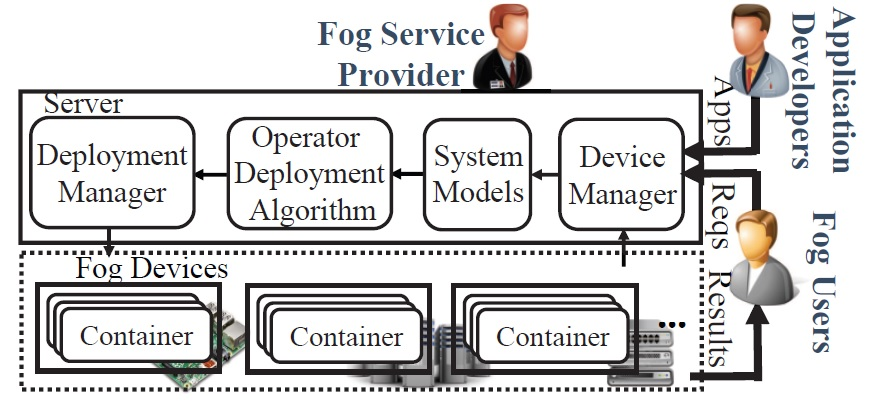
\includegraphics[width=0.40\textwidth]{fig/architecture.eps}
    \caption{High-level system architecture with a network of MANEs.}
\vspace{-0.1cm}
    \label{architecture} 
\end{figure}

Figure. ~\ref{architecture} show our architecture of the whole system. It is composed of a sender, some clients, some P4-based MANEs, some regular switches, and a ONOS controller connects those MANEs. The ONOS controller forms a control plane disassociate from the data plane. 
